\documentclass[a4j,dvipdfmx]{jarticle}
%----------------------------------------------------------------------
\usepackage{graphicx}
\usepackage{amsmath}
\usepackage{amssymb}
\usepackage{bm}
\usepackage{fancybox}
\usepackage{fancyhdr}
\usepackage{lastpage}
\usepackage{color}
\usepackage{multicol}
\usepackage{listings,jlisting}
%----------------------------------------------------------------------
\setlength{\topmargin}{-0.5in}
%\addtolength{\headheight}{1cm}
%%\setlength{\headsep}{0mm}
%\setlength{\oddsidemargin}{-0.5in}
%%\setlength{\evensidemargin}{-0.5in}
%\addtolength{\textwidth}{1.5in}
\addtolength{\textheight}{1in}
%----------------------------------------------------------------------
%\setlength{\columnsep}{2zw}
%\setlength{\columnseprule}{0.4pt}
%----------------------------------------------------------------------
\pagestyle{fancy}
\lhead{2016/04/05}
\rhead{配布資料(\thepage / \pageref{LastPage})}
\cfoot{}
\chead{\textgt{システムプログラミング2 第1回}}
%----------------------------------------------------------------------
\begin{document}
\def\lstlistingname{リスト}
\lstset{language=C,
  numbers=left,
  basicstyle={\small\ttfamily},
  columns=[l]{fullflexible},
  keepspaces=true,
  frame=shadowbox,
  commentstyle=\slshape
}
%----------------------------------------------------------------------

%\begin{figure}[hbtp]
%\begin{center}
%\includegraphics[height=2.5cm]{state.pdf}
%\caption{単語の長さをカウントするアルゴリズム}
%\end{center}
%\end{figure}

今回は、ファイルの読み書きについて学ぶ。
教科書の P.194 〜 P.202 の内容が対応する。
3年次に作ったプログラムは{\tt stdin}から入力({\tt getchar()})し、
{\tt stdout}へ出力({\tt putchar()}、{\tt printf()})するものだった。
今回は、任意のファイルを読み書きするプログラムを作る。

C言語では、ファイルをバイトの1次元配列(バイトストリーム)と考える。
{\tt stdin}や{\tt stdout}、{\tt stderr}もバイトストリームだったので、
これらと同様の手順でファイルも扱うことができる。

\begin{enumerate}
\item ファイルのオープン({\tt fopen()}関数)\\
{\tt stdin}や{\tt stdout}、{\tt stderr}は、
特別に予めオープンされたファイルである。
普通のファイルはプログラム内で明示的にオープンする必要がある。
{\tt fopen()}がファイルをオープンする関数である。

\begin{multicols}{2}
\begin{lstlisting}[numbers=none]
#include <stdio.h>
FILE *fopen(char *fname, char *mode);

例: // バイナリファイルをリードオープン
     FILE *fp;       // ファイルポインタ
     fp = fopen("a.dat", "rb");
     if (fp==NULL) {   // エラーチェック
\end{lstlisting}

fname:ファイル名\\
mode :\\
  "r":読み(read)\\
  "w":書き(write) + "b":バイナリ\\
  "a":追加(append)\\
返り値:FILE構造体を指すポインタ
\end{multicols}

%\begin{figure}[hbtp]
\begin{center}
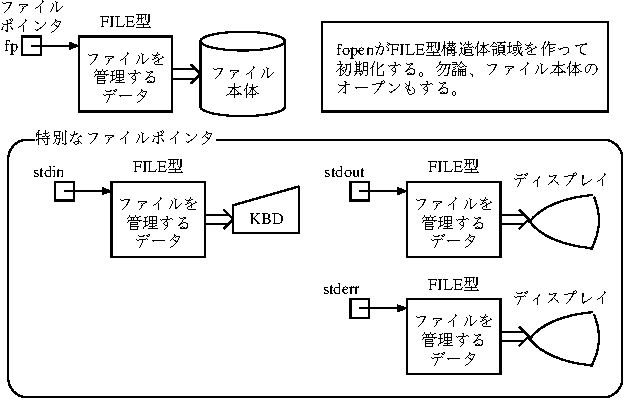
\includegraphics[scale=1.3]{FILE.pdf}
%\caption{単語の長さをカウントするアルゴリズム}
\end{center}
%\end{figure}

\item ファイル入出力

\begin{enumerate}
\item 1文字入力({\tt getc()}関数 --- {\tt getchar()}のファイル版 ---)

\begin{multicols}{2}
\begin{lstlisting}[numbers=none]
#include <stdio.h>
int getc(FILE *fp);
// getchar()は次のように定義できる
// #define getchar()  getc(stdin)
\end{lstlisting}
\columnbreak

{\tt getc}は、ファイルから読んだ1バイトの値(0〜255)を返す。
{\tt EOF}になると$-1$を返す。({\tt getchar()}と同様)
\end{multicols}

\begin{multicols}{2}
\begin{lstlisting}[numbers=none]
例:ファイルから1バイト読む
FILE *fp = fopen("a.txt", "r");
int ch;                  // int 型!!
ch = getc(fp);
\end{lstlisting}
\columnbreak

左の例は、{\tt a.txt}ファイルの最初の1バイトを変数{\tt ch}に読み込む。
\end{multicols}

\item 1文字出力({\tt putc()}関数 --- {\tt putchar()}のファイル版 --- )
\begin{multicols}{2}
\begin{lstlisting}[numbers=none]
#include <stdio.h>
int putc(int c, FILE *fp);
// putchar()は次のように定義できる
// #define putchar()  putc(stdout)
\end{lstlisting}
\columnbreak

\begin{lstlisting}[numbers=none]
例:ファイルに文字「a」を書き込む
FILE *fp = fopen("a.txt", "w");
putc('a', fp);
\end{lstlisting}
\end{multicols}

\item 1行入力({\tt fgets()}関数)

\begin{multicols}{2}
\begin{lstlisting}[numbers=none]
#include <stdio.h>
char *fgets(char *buf,
            int size, FILE *fp);
// fgets は EOF で NULL を返す
\end{lstlisting}
\columnbreak

buf  : 1行入力バッファ\\
size : バッファの大きさ\\
fp   : ファイルポインタ
\end{multicols}

\begin{multicols}{2}
\begin{lstlisting}[numbers=none]
例:ファイルから1行読む
FILE *fp = fopen("a.txt", "r");
char buf[100];
fgets(buf, 100, fp);
\end{lstlisting}
\columnbreak

左の例は、{\tt a.txt}ファイルの最初の1行を{\tt buf}に入力する。
{\tt buf}の最後には、\verb/"\n\0"/が格納される。
\end{multicols}

\item 1行出力({\tt fputs()}関数 --- {\tt puts()}のファイル版 ---)
\begin{multicols}{2}
\begin{lstlisting}[numbers=none]
#include <stdio.h>
int fputs(char *buf, FILE *fp);
// エラー時に EOF を返す
// bufは'\0'で終わる文字列
\end{lstlisting}
\columnbreak

\begin{lstlisting}[numbers=none]
例:ファイルに文字列「abc\n」を書き込む
FILE *fp = fopen("a.txt", "w");
fputs("abc\n", fp);
\end{lstlisting}
\end{multicols}

\item 書式付き出力({\tt fprintf()}関数 --- {\tt printf()}のファイル版 --- )
\begin{multicols}{2}
\begin{lstlisting}[numbers=none]
#include <stdio.h>
int fprintf(FILE *fp,
            char *format, ...);
\end{lstlisting}
\columnbreak

\begin{lstlisting}[numbers=none]
例:ファイルにデータを書き込む
FILE *fp = fopen("a.txt", "w");
fprintf(fp, "%d,%d\n", x, y);
\end{lstlisting}
\end{multicols}
\end{enumerate}

\item ファイルのクローズ({\tt fclose()}関数)
\begin{lstlisting}[numbers=none]
#include <stdio.h>
int fclose(FILE *fp);
\end{lstlisting}

\item エラーメッセージの出力({\tt perror()}関数)

直近に発生したエラーを説明するメッセージを{\tt stderr}に出力する。
\begin{lstlisting}[numbers=none]
#include <stdio.h>
void perror(char *msg);  // msg はエラーメッセージの先頭に付加する文字列

例:ファイルオープンに失敗のエラー処理
     fp = fopen("a.txt", "r");
     if (fp==NULL) {
       perror("a.txt");  // "a.txt: No such file or directory" などと表示
       exit(1);
     }
\end{lstlisting}

\item プログラム例

\lstinputlisting[numbers=none]{mycat.c}

実行例:

\begin{lstlisting}[numbers=none]
$ mycat                      <--- ファイルが指定されていない場合
aaaa                         <--- 入力
aaaa                         <--- 出力
bbbb                         <--- 入力
bbbb                         <--- 出力
^D                           <--- EOF
$ mycat a.txt
hello                        <--- a.txt の内容を表示
$ mycat b.txt
world                        <--- b.txt の内容を表示
$ mycat a.txt b.txt
hello                        <--- a.txt の内容を表示
world                        <--- b.txt の内容を表示
$
\end{lstlisting}

\item 演習(#1) 〆切 4月11日
\begin{enumerate}
\item {\tt mycp}コマンド

ファイルをコピーするプログラム{\tt mycp}を作りなさい。
{\tt mycp}は、{\tt cp}コマンドの簡易版です。
次のように使います。
エラー処理もすること。
\begin{lstlisting}[numbers=none]
$ mycp file1 file2           <--- file1 の内容を file2 にコピー
\end{lstlisting}

\item {\tt mydiff}コマンド

二つのファイルを比較して、違っている最初の行と
行番号を印刷するプログラムを書きなさい。
処理できる1行の最大の長さは自分で決めてい良い。
次のように使います。
エラー処理もすること。
\begin{lstlisting}[numbers=none]
$ mydiff a.txt b.txt         <--- a.txt と b.txt を比較
2行目
> world
< World
$
\end{lstlisting}
\end{enumerate}

\end{enumerate}
\end{document}
